\documentclass[crop]{standalone}
\usepackage{tikz}
\usepackage{pgfplots}
\pgfplotsset{compat=1.15}
\usepackage[]{amsmath}
\usepackage[]{libertine-type1}
\usepackage[libertine]{newtxmath}
\usepackage[]{bm}
\usepackage[]{physics}
\usepackage[]{xstring}
% Macros for greek letters in roman style, in math mode
\DeclareRobustCommand{\mathup}[1]{%
\begingroup\ensuremath\changegreek\mathrm{#1}\endgroup}
\DeclareRobustCommand{\mathbfup}[1]{%
\begingroup\ensuremath\changegreek\bm{\mathrm{#1}}\endgroup}


\makeatletter
\def\changegreek{\@for\next:={%
        alpha,beta,gamma,delta,epsilon,zeta,eta,theta,iota,kappa,lambda,mu,nu,%
        xi,pi,rho,sigma,tau,upsilon,phi,chi,psi,omega,varepsilon,varpi,%
    varrho,varsigma,varphi}%
\do{\expandafter\let\csname\next\expandafter\endcsname\csname\next up\endcsname}}
\makeatother

% Define vectors in bold, roman, lowercase font
\newcommand{\vct}[1]{\ensuremath{\mathbfup{\MakeLowercase{#1}}}}

% Define unit vectors in bold, roman, lowercase font, with hats
\newcommand{\uvct}[1]{\ensuremath{\mathbfup{\hat{\MakeLowercase{#1}}}}}

% Define matrices in bold, roman, uppercase font
\newcommand{\mtrx}[1]{\ensuremath{\mathbfup{\MakeUppercase{#1}}}}
\usetikzlibrary{%
    angles,%
    arrows.meta,%
    backgrounds,%
    calc,%
    decorations,%
    fit,%
    hobby,%
    patterns,%
    positioning,%
    quotes
}



\begin{document}


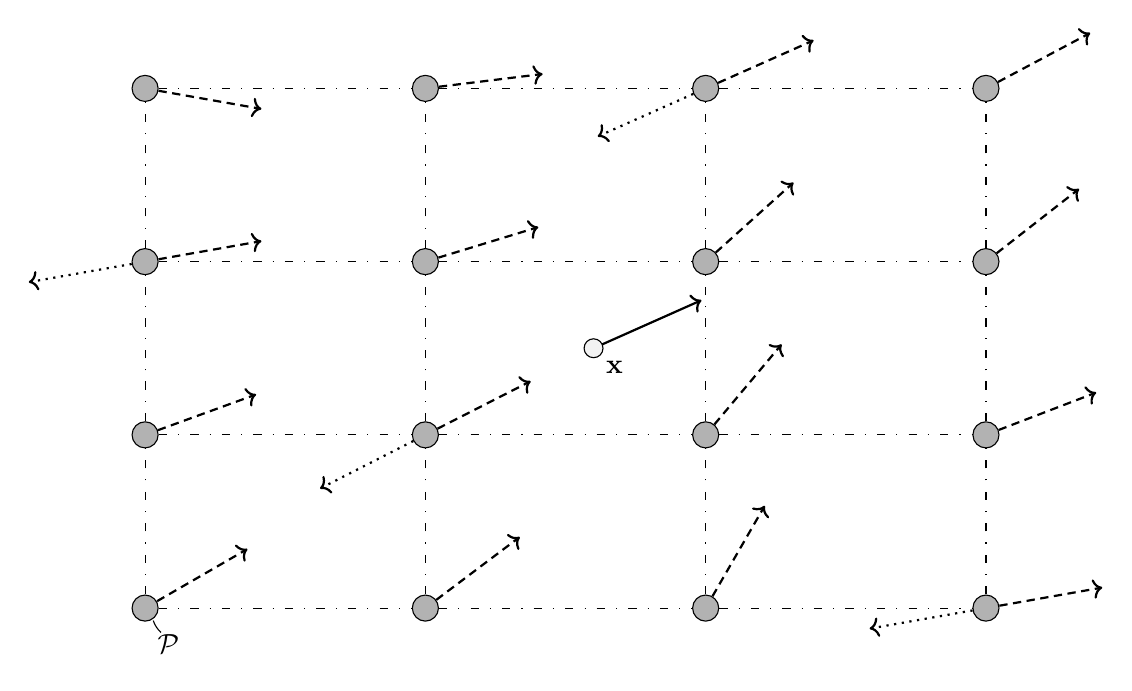
\begin{tikzpicture}
    \coordinate (pivot) at (0,0);
    % Form factors of the fluid cell
    \pgfmathsetmacro{\sy}{2.2};
    \pgfmathsetmacro{\sx}{1.618*\sy};
    % Radii of fluid elements
    \pgfmathsetmacro{\r}{0.4};

    % Draw fluid elements in interpolation voxel
    \foreach \i in {0,...,3}%
    {%
        \foreach \j in {0,...,3}%
        {%
            {\pgfmathtruncatemacro{\label}{\i-4*\j+13}
            \node[circle,draw,fill=gray!60,stroke=black!80,minimum size =1.5*\r] (\i\j) at ($(pivot) + (\i*\sx,\j*\sy)$) {};}
        }
    }

    % Connect fluid elements in interpolation voxel by dashed lines
    \foreach \i in {0,...,3}%
    {%
        \foreach \j [count=\ji] in {0,...,2}%
        {%
            \draw[stroke=black!80,thin,loosely dashdotted] (\i\j)--(\i\ji) (\j\i) -- (\ji\i);
        }
    }

    % Draw fluid element at which interpolated value is sought
    \coordinate (pos) at ($(pivot) + (1.6*\sx,1.5*\sy)$);
    \draw[circle,fill=gray!10,stroke=black!80,minimum size=0.3*\r] (pos) circle (0.3*\r);
    \node at (pos) [below right=1pt and 1pt] {$\vct{x}$};

    % Indicate pivot vector
    \node [below right = 6pt and 1pt of pivot] (pivotmrk) {$\mathcal{P}$};
    \draw[stroke=black!80] ($(pivotmrk)!0.32!(pivot)$) to [out=135,in=-70] ($(pivotmrk)!0.65!(pivot)$);

    % Draw unit vectors at background layer in order to reduce foreground clutter
    \begin{scope}[on background layer]
    % Define scale of unit eigenvectors
    \pgfmathsetmacro{\vl}{1.5};
    % Draw interpolated vector
    \draw[->,stroke=black!80,thick] (pos) to ($(pos) + ({\vl*cos(24)},{\vl*sin(24)})$);

    % Draw unit vector at pivot
    \draw[->,stroke=black!80,densely dashed,thick] (pivot) to ($(pivot) + ({\vl*cos(30)},{\vl*sin(30)})$);

    % Draw unit vectors at remaining grid points, some of which are
    % rotated in advance
    \draw[->,stroke=black!80,densely dashed,thick] (01) to ($(01) + ({\vl*cos(20)},{\vl*sin(20)})$);
    \draw[->,stroke=black!80,dotted, thick] (02) to ($(02) + ({\vl*cos(190)},{\vl*sin(190)})$); % Needs to be flipped
    \draw[->,stroke=black!80,densely dashed,thick] (02) to ($(02) + ({\vl*cos(10)},{\vl*sin(10)})$);
    \draw[->,stroke=black!80,densely dashed,thick] (03) to ($(03) + ({\vl*cos(-10)},{\vl*sin(-10)})$);
    \draw[->,stroke=black!80,densely dashed,thick] (10) to ($(10) + ({\vl*cos(37)},{\vl*sin(37)})$);
    \draw[->,stroke=black!80,dotted,thick] (11) to ($(11) + ({\vl*cos(207)},{\vl*sin(207)})$); % Needs to be flipped
    \draw[->,stroke=black!80,densely dashed,thick] (11) to ($(11) + ({\vl*cos(27)},{\vl*sin(27)})$);
    \draw[->,stroke=black!80,densely dashed,thick] (12) to ($(12) + ({\vl*cos(17)},{\vl*sin(17)})$);
    \draw[->,stroke=black!80,densely dashed,thick] (13) to ($(13) + ({\vl*cos(07)},{\vl*sin(07)})$);
    \draw[->,stroke=black!80,densely dashed,thick] (20) to ($(20) + ({\vl*cos(60)},{\vl*sin(60)})$);
    \draw[->,stroke=black!80,densely dashed,thick] (21) to ($(21) + ({\vl*cos(50)},{\vl*sin(50)})$);
    \draw[->,stroke=black!80,densely dashed,thick] (22) to ($(22) + ({\vl*cos(42)},{\vl*sin(42)})$);
    \draw[->,stroke=black!80,dotted,thick] (23) to ($(23) + ({\vl*cos(204)},{\vl*sin(204)})$); % Needs to be flipped
    \draw[->,stroke=black!80,densely dashed,thick] (23) to ($(23) + ({\vl*cos(24)},{\vl*sin(24)})$);
    \draw[->,stroke=black!80,dotted,thick] (30) to ($(30) + ({\vl*cos(190)},{\vl*sin(190)})$); % Needs to be flipped
    \draw[->,stroke=black!80,densely dashed,thick] (30) to ($(30) + ({\vl*cos(10)},{\vl*sin(10)})$);
    \draw[->,stroke=black!80,densely dashed,thick] (31) to ($(31) + ({\vl*cos(21)},{\vl*sin(21)})$);
    \draw[->,stroke=black!80,densely dashed,thick] (32) to ($(32) + ({\vl*cos(38)},{\vl*sin(38)})$);
    \draw[->,stroke=black!80,densely dashed,thick] (33) to ($(33) + ({\vl*cos(28)},{\vl*sin(28)})$);




    \end{scope}




\end{tikzpicture}
\end{document}
